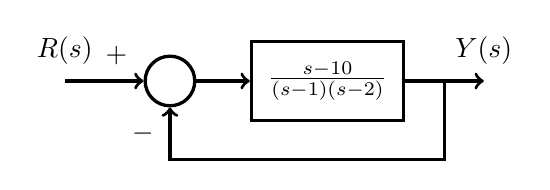
\begin{tikzpicture}[very thick,
sysblock/.style={draw,rectangle,inner sep=6pt,minimum width=1.25cm,minimum height=1.0cm,very thick},
summer/.style={circle,draw,very thick}]

\draw (0,0) node[summer] (sum) {\rule{10pt}{0pt}};
\draw (2,0) node[sysblock] (C) {$\frac{s-10}{(s-1)(s-2)}$};

\draw[<-] (sum.180) node[above left=2pt] {$+$} -- ++(-1,0) node[above=2pt] {$R(s)$};
\draw[->] (sum.0) -- (C.180);
\draw[->] (C.0) -- ++(0.5,0) -- ++(0,-1)  -| (sum.-90) node[below left=2pt] {$-$};
\draw[->] (C.0) ++(0.5,0) -- ++(0.5,0) node[above=2pt] {$Y(s)$};

\end{tikzpicture}